\section{Motion Estimation and Video Coding}




\begin{questionbox}{Domanda 74}
\textbf{motion estimation}: give the principles of the block matching approach. Give at least one cost function. [Bonus]. Discuss the regularization issue.
\end{questionbox}


Block matching splits a frame into blocks $B_{p,q}$ and searches a reference frame for the most similar block inside a search window.

The best displacement is:


$$
(\hat{i},\hat{j})=\arg\min_{(i,j)\in W}J(i,j)
$$


SSD:


$$
J_{\text{SSD}}(i,j)=
\sum_{(n,m)\in B_{p,q}}
[f(n,m,k)-f(n-i,m-j,h)]^2
$$


SAD:


$$
J_{\text{SAD}}(i,j)=
\sum_{(n,m)\in B_{p,q}}
|f(n,m,k)-f(n-i,m-j,h)|
$$


Regularized cost:


$$
J_{\text{REG}}(i,j)=
\|\vec{f}_k(B_{p,q})-\vec{f}_h(B_{p-i,q-j})\|_p^p
+\lambda R(i,j)
$$


Regularization penalizes expensive or irregular motion vectors and balances prediction quality with motion-vector coding \textbf{rate}.



\begin{questionbox}{Domanda 75}
Discuss the advantages and the disadvantages of Intra, Predictive, and Bidirectional images in a GOP for video coding.
\end{questionbox}



\begin{center}
\begin{tabular}{ | l | l | l | l | }
\hline
\textbf{Frame type} & \textbf{Prediction} & \textbf{Advantages} & \textbf{Disadvantages} \\
\hline
I & Intra only & Random access, error reset, no ME & High rate, lower compression \\
\hline
P & From previous anchor frames & Good compression, moderate delay & ME/MC complexity, error propagation \\
\hline
B & From past and future frames & Best compression & Highest complexity, structural delay, not ideal for low latency \\
\hline
\end{tabular}
\end{center}
GOP structure controls compression efficiency, delay, random access interval and error propagation.



\begin{questionbox}{Domanda 76}
(ME) Describe the difference between “motion field” and “optical flow”.
\end{questionbox}


\textbf{Motion field} is the projection of actual 3D scene motion onto the image plane.

\textbf{Optical flow} is the apparent motion of brightness patterns in the image. They often coincide, but not always, because illumination changes, occlusions and texture ambiguities can break the relation.



\begin{questionbox}{Domanda 77}
(ME) Explain the Horn and Schunck algorithm’s core principle for dense optical flow estimation.
\end{questionbox}


The optical flow constraint is:


$$
u f_x + v f_y + f_t = 0
$$


Horn-Schunck estimates dense flow by minimizing data attachment plus smoothness:


$$
J=
\iint_{\mathcal{R}}(u f_x+v f_y+f_t)^2\,dxdy
+\lambda\iint_{\mathcal{R}}(\|\nabla u\|^2+\|\nabla v\|^2)\,dxdy
$$


The first term enforces brightness consistency; the second term regularizes the flow field so neighboring vectors vary smoothly.



\begin{questionbox}{Domanda 78}
(ME) Discuss the \textbf{\textbf{rate}-\textbf{distortion}} trade-off when selecting block sizes in \textbf{motion estimation}.
\end{questionbox}


\textbf{motion estimation} can use:


$$
J(v)=d(B_k^{(p)},B_h^{(p+v)})+\lambda_{ME}R(v)
$$


Large blocks:

\begin{itemize}
  \item fewer motion vectors,
  \item lower side information and complexity,
  \item worse fit near object boundaries.
\end{itemize}

Small blocks:

\begin{itemize}
  \item better prediction and lower \textbf{distortion},
  \item more motion vectors and partition bits,
  \item higher complexity.
\end{itemize}



\begin{questionbox}{Domanda 79}
(ME) Which of the following is a disadvantage of using the Sum of Squared Differences (SSD) as a matching criterion?
\end{questionbox}


SSD squares errors, so outliers dominate the cost. Illumination changes, noise or occlusions can produce irregular motion vectors. SAD is often more robust and cheaper.



\begin{questionbox}{Domanda 80}
(ME) What is the main benefit of the Hexagon Search strategy compared to Full Search?
\end{questionbox}


Full search tests all candidate vectors and is optimal within the window, but expensive. Hexagon search tests a small hexagonal pattern iteratively and greatly reduces candidate evaluations. It is faster but not guaranteed globally optimal.



\begin{questionbox}{Domanda 81}
(ME) What does an affine motion model allow that a pure translational model does not?
\end{questionbox}


Translation uses only a constant displacement. Affine motion can also represent rotation, zoom and shear:


$$
\vec{v}(p)=\vec{b}+Bp
=
\begin{bmatrix}b_1\\b_2\end{bmatrix}
+
\begin{bmatrix}b_3&b_4\\b_5&b_6\end{bmatrix}p
$$


If $B=0$, it reduces to pure translation / block matching.



\begin{questionbox}{Domanda 82}
Draw the block diagram of a hybrid video encoder (\textbf{motion estimation}/compensation + \textbf{DCT} + \textbf{quantization} + \textbf{entropy} coding + reconstruction loop with frame buffer). Explain why the encoder contains an internal decoder.
\end{questionbox}


A hybrid video encoder codes the prediction residual, not usually the whole frame:

\begin{figure}[H]
\centering
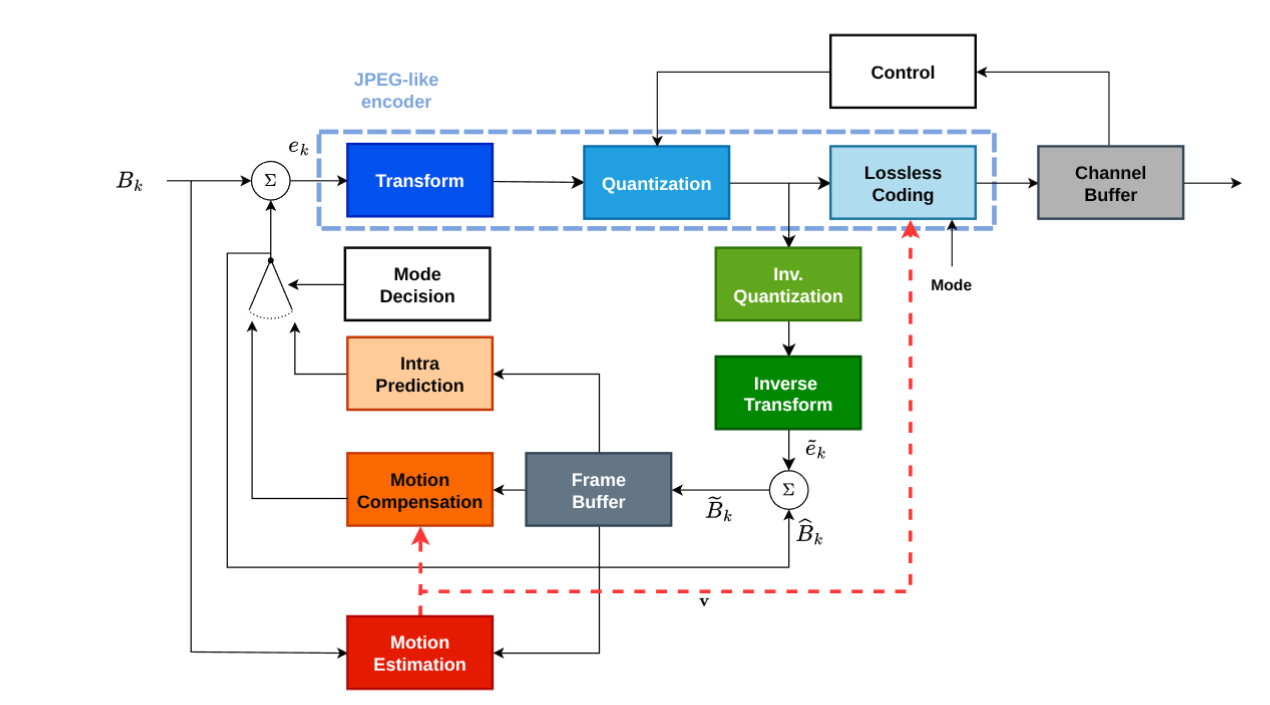
\includegraphics[width=0.75\textwidth]{images/Hybrid_video_encoder.png}
\caption{Hybrid video encoder}
\end{figure}\begin{tcolorbox}[colback=white, colframe=gray!50, height=4.5cm, sharp corners]
\end{tcolorbox}

This scheme combines inter/\textbf{intra prediction} with JPEG-like residual coding. Mode decision selects the predictor, transform and \textbf{quantization} encode the residual, \textbf{lossless} coding creates the bitstream, and the inverse \textbf{quantization}/inverse transform path reconstructs the same block that will be stored in the frame buffer for later \textbf{motion compensation}.

The encoder contains an internal decoder because future predictions must be built from exactly the same reconstructed frames available at the decoder. If the encoder predicted from original frames while the decoder predicted from reconstructed frames, their references would diverge and drift would propagate through the video.



\begin{questionbox}{Domanda 83}
(VCP) Why is the temporal prediction error usually more efficient to encode than the original video signal?
\end{questionbox}


\begin{figure}[H]
\centering
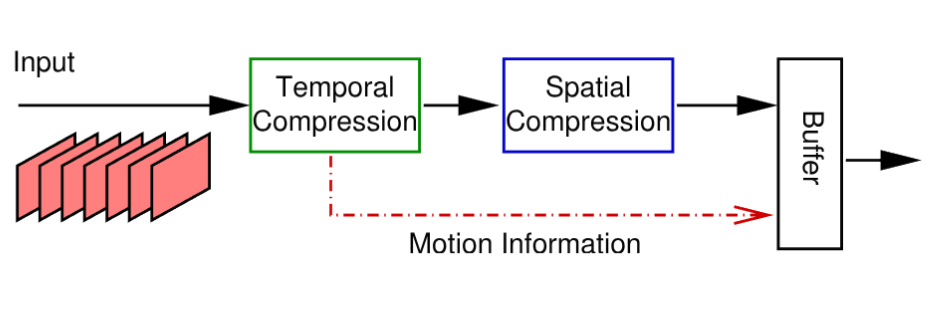
\includegraphics[width=0.75\textwidth]{images/Video_coding_principles.png}
\caption{Video coding principles}
\end{figure}\begin{tcolorbox}[colback=white, colframe=gray!50, height=4.5cm, sharp corners]
\end{tcolorbox}

This high-level video coding scheme separates temporal compression from spatial compression. Temporal compression exploits similarity between frames and produces motion information, while spatial compression removes redundancy inside the prediction residual; the buffer then regulates the coded stream \textbf{rate}.

Neighboring video frames are highly correlated. Motion-compensated prediction estimates the current block from reference frames, then encodes only:


$$
e=x-x_p
$$


The residual is usually lower-energy and more sparse than the original frame, so transform \textbf{quantization} and \textbf{entropy} coding are more efficient.



\begin{questionbox}{Domanda 84}
(VCP) Describe the function of the “Mode Selection” step in a hybrid video encoder.
\end{questionbox}


Mode selection chooses the coding mode that minimizes \textbf{\textbf{rate}-\textbf{distortion}} cost:


$$
J = D+\lambda R
$$


For blocks:


$$
D=\sum_{k=1}^{K}D_k(i_k,Q),
\quad
R=\sum_{k=1}^{K}R_k(i_k,Q)
$$



$$
J(\vec{i},Q,\lambda)=D(\vec{i},Q)+\lambda R(\vec{i},Q)
$$


The encoder usually performs suboptimal block-wise minimization:


$$
i_k^\star=\arg\min_{i_k}J_k(i_k,Q,\lambda)
$$


Typical empirical choices:


$$
\text{MPEG-2: } \lambda=aQ^2+b
$$



$$
\text{H.264: } \lambda=c\cdot2^{dQ+e},
\quad
\lambda_{ME}=\sqrt{\lambda}
$$




\begin{questionbox}{Domanda 85}
(VCP) How does the “Channel Buffer” controller manage the trade-off between target \textbf{rate} and video quality?
\end{questionbox}


The channel buffer controls the \textbf{quantization} step to meet target \textbf{rate}:

\begin{itemize}
  \item if buffer occupancy is too high, increase \textbf{quantization} step to reduce \textbf{rate};
  \item if buffer occupancy is too low, decrease \textbf{quantization} step to improve quality.
\end{itemize}

This avoids overflow/underflow while keeping quality as high as possible.



\begin{questionbox}{Domanda 86}
(VCP) What is the primary role of an “I-frame” in a GOP structure?
\end{questionbox}


An I-frame is intra-coded and independently decodable. It provides random access, starts a GOP and limits temporal error propagation.



\begin{questionbox}{Domanda 87}
(VCP) In the context of \textbf{motion vector} coding, why is a Median Predictor (MVP) used?
\end{questionbox}


Neighboring motion vectors are correlated. The median predictor estimates the current vector from adjacent blocks, then the encoder sends only the motion-vector difference:


$$
\text{MVD} = \text{MV} - \text{MVP}
$$


This difference is usually small and cheaper to encode.



\begin{questionbox}{Domanda 88}
(VCP) What happens in the decoder when it receives an “Inter-coded” block?
\end{questionbox}


\begin{figure}[H]
\centering
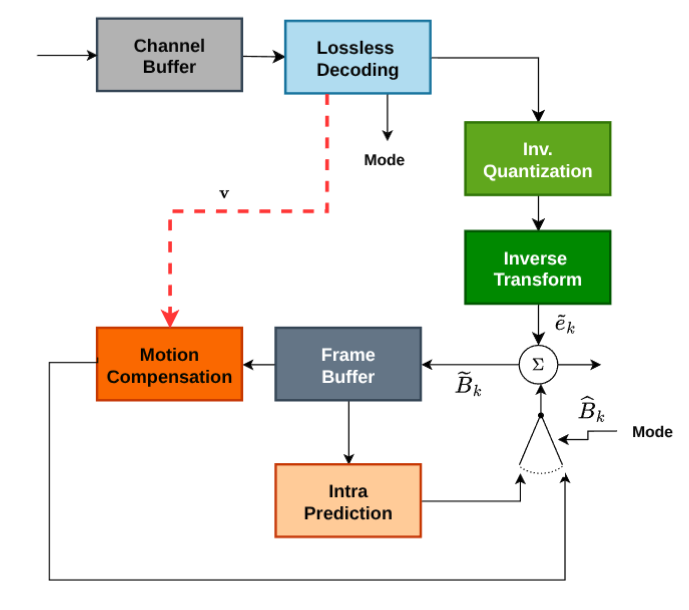
\includegraphics[width=0.75\textwidth]{images/Hybrid_video_decoder.png}
\caption{Hybrid video decoder}
\end{figure}\begin{tcolorbox}[colback=white, colframe=gray!50, height=4.5cm, sharp corners]
\end{tcolorbox}

The hybrid decoder reverses only the normative part of the encoder. \textbf{entropy} decoding recovers mode information, motion vectors and quantized residuals; inverse \textbf{quantization} and inverse transform reconstruct the residual; \textbf{intra prediction} or \textbf{motion compensation} builds the predictor, which is added to the residual and stored in the frame buffer.

The decoder reads side information: mode, reference index and \textbf{motion vector}. It fetches the predictor from the decoded frame buffer, decodes the residual, then reconstructs:


$$
\hat{x}=\text{prediction}+\hat{e}
$$


---


